\documentclass[12pt]{article}

\usepackage[margin = .8in]{geometry}
\usepackage{amsmath}
\usepackage{graphicx}
\usepackage{multicol, enumerate, tabularx}

\usepackage{adjustbox}

\usepackage{fancyhdr}
\pagestyle{fancy}

\lhead{Math F113X: Numbers and Society}
\rhead{Date: \hspace{1in}}

\usepackage{tikz}
\usetikzlibrary{calc,trees,positioning,arrows,fit,shapes,through, backgrounds}
\usetikzlibrary{patterns}

\usetikzlibrary{decorations.markings}
\usetikzlibrary{arrows}

\usepackage{pgfplots}

\usepackage{longtable}
\usepackage{tabularx}

\newcommand{\ds}{\displaystyle}
\newcommand{\ans}[1][1in]{\rule{#1}{.5pt}}

\newcommand{\points}[1]{(#1 points.)}		% Trying to be lazy.

\usepackage{array}
\newcolumntype{L}[1]{>{\raggedright\let\newline\\\arraybackslash\hspace{0pt}}m{#1}}
\newcolumntype{C}[1]{>{\centering\let\newline\\\arraybackslash\hspace{0pt}}m{#1}}
\newcolumntype{R}[1]{>{\raggedleft\let\newline\\\arraybackslash\hspace{0pt}}m{#1}}
\newcommand{\red}[1]{\textcolor{red}{#1}}

\newcommand{\be}{\begin{enumerate}}
\newcommand{\ee}{\end{enumerate}}

%\topmargin -1in
%\textheight 9.5in
%\oddsidemargin -0.3in
%\evensidemargin \oddsidemargin
%\pagestyle{empty}
%%\marginparwidth 0.5in
%\textwidth 7in
%\parindent 0in

%--------------------------------------------------------------------------------------------------------------------------------------------------------------------------
%						Document
%--------------------------------------------------------------------------------------------------------------------------------------------------------------------------


\begin{document}
%\pagestyle{fancy}
\begin{center}
{\Large  Worksheet 12 (Graph Theory 4): Euler Paths and Circuits}
\end{center}



\noindent \textbf{Group Names:} \hrulefill \\
%-------------------------------------------------------------------------------------------------------------
%						Assignment
%-----------------------------------------------------------------------------------------------------
\begin{enumerate}

\item For each of the following graphs, do the following:
\be[(i)]
\item Highlight all the vertices of odd degree.
\item Determine whether it has an Euler path or an Euler circuit. If it has an Euler path or circuit, circle the correct choice. If it has neither an Euler path nor an Euler circuit, explain why. 
\ee
\be[ {path} $\quad$ {circuit} $\quad$ ne{i}ther $\quad$]
\item 
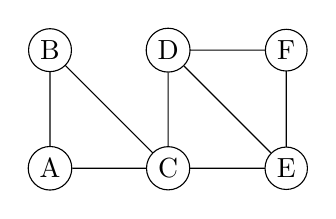
\begin{tikzpicture}[baseline=(current bounding box.center), scale=.5]
\tikzstyle{every node}=[circle, draw, fill=black!0,
                        inner sep=2pt, minimum width=10pt]
\draw (0,0) node (A) {A} -- (0,3) node (B) {B}
-- (3,0) node (C) {C} --(6,0) node (E) {E} -- (6,3) node (F) {F} -- (3,3) node (D) {D};
\draw (A) --(C) -- (D)--(E);
\end{tikzpicture}

\vfill
\item 
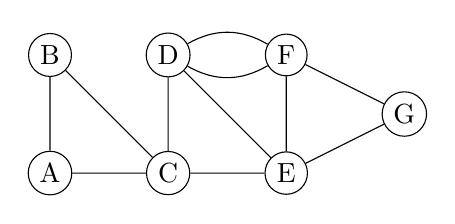
\begin{tikzpicture}[baseline=(current bounding box.center), scale=.5]
\tikzstyle{every node}=[circle, draw, fill=black!0,
                        inner sep=2pt, minimum width=10pt]
\path (0,0) node (A) {A} ;
\node (B)  at (0,3) {B};
\node (C) at (3,0) {C} ;
\node (E) at (6,0) {E} ;
\node (F) at (6,3)  {F} ;
\node (D) at (3,3)  {D};
\node (G) at (9, 1.5) {G};
\draw (A) -- (B) -- (C) -- (D) edge[bend right=30] (F);
\draw  (F)--(G) -- (E) -- (F) edge[bend right=30] (D);
\draw (D)-- (E) --(C) --(A);
\end{tikzpicture}

\vfill

\item 
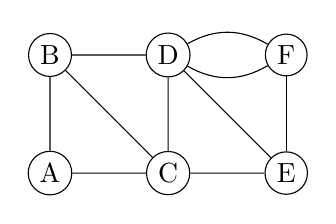
\begin{tikzpicture}[baseline=(current bounding box.center), scale=.5]
\tikzstyle{every node}=[circle, draw, fill=black!0,
                        inner sep=2pt, minimum width=10pt]
\path (0,0) node (A) {A} ;
\node (B)  at (0,3) {B};
\node (C) at (3,0) {C} ;
\node (E) at (6,0) {E} ;
\node (F) at (6,3)  {F} ;
\node (D) at (3,3)  {D};
\draw (A) -- (B) -- (C) -- (D) edge[bend right=30] (F);
\draw  (F) -- (E) -- (F) edge[bend right=30] (D);
\draw (B)--(D)-- (E) --(C) --(A);
\end{tikzpicture}


\item 
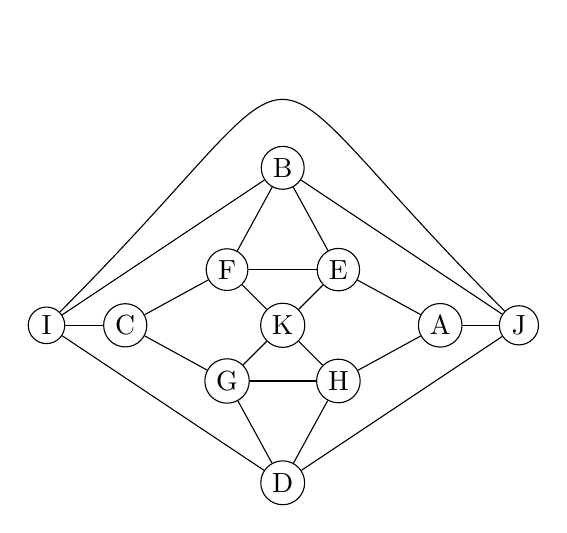
\begin{tikzpicture}[baseline=(current bounding box.center),]
\tikzstyle{vertex}=[circle, draw, inner sep=2pt]%, minimum size=6pt]

\tikzstyle{every node} = [vertex];
\node (A) at (0:2) {A};
\node (B) at (90:2) {B};
\node (C) at (180:2) {C};
\node (D) at (270:2) {D};
\node (O) at (0,0){K};
\node (E) at (45:1) {E};
\node (F) at (45+90:1){F};
\node (G) at (45+180:1){G};
\node (H) at (45+270:1){H};
\node[left of = C] (I) {I};
\node [right of = A] (J) {J};
\draw (B) -- (I) -- (D) -- (J)--(B);
\draw (A) -- (E) -- (B) -- (F) -- (C) -- (G) -- (D) -- (H) -- (A);
\draw (E) -- (O) -- (G) (F) --(O) --(H);
\draw (A) -- (J) (C) -- (I);
\draw (I) to[looseness = 3, distance = 2in] (J);
\draw (E) -- (F)  (G) -- (H);
\end{tikzpicture}

\ee 


\newpage

\item Find an Euler circuit on the following graph. Draw it next to the edges of the graph so it is clear what the circuit should be, and list the vertices of the circuit in order.

\bigskip

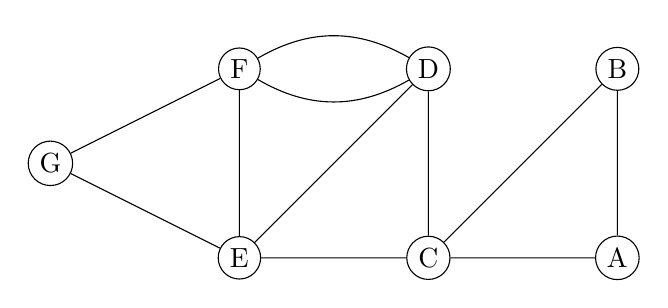
\begin{tikzpicture}[baseline=(current bounding box.center), scale=.8]
\tikzstyle{every node}=[circle, draw, fill=black!0,
                        inner sep=2pt, minimum width=10pt]
\path (0,0) node (A) {A} ;
\node (B)  at (-0,3) {B};
\node (C) at (-3,0) {C} ;
\node (E) at (-6,0) {E} ;
\node (F) at (-6,3)  {F} ;
\node (D) at (-3,3)  {D};
\node (G) at (-9, 1.5) {G};
\draw (A) -- (B) -- (C) -- (D) edge[bend right=30] (F);
\draw  (F)--(G) -- (E) -- (F) edge[bend right=30] (D);
\draw (D)-- (E) --(C) --(A);
\end{tikzpicture}

\bigskip


circuit: \hrulefill

\item 
\be
\item This graph has two vertices of odd degree. What are they? \ans
\item Find an Euler path. Draw it next to the edges of the graph so it is clear what the path should be, and list the vertices of the path in order.
\ee

\bigskip

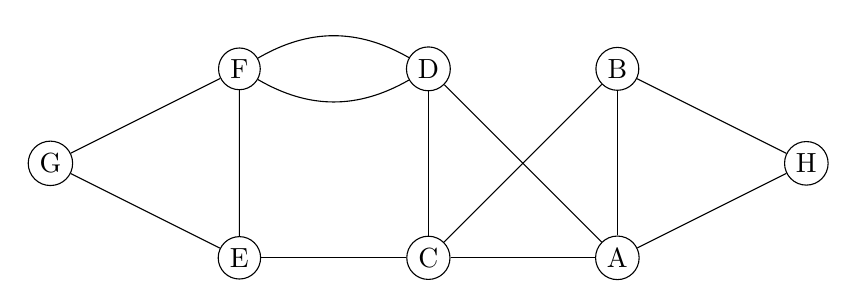
\begin{tikzpicture}[baseline=(current bounding box.center), scale=.8]
\tikzstyle{every node}=[circle, draw, fill=black!0,
                        inner sep=2pt, minimum width=10pt]
\path (0,0) node (A) {A} ;
\node (B)  at (-0,3) {B};
\node (C) at (-3,0) {C} ;
\node (E) at (-6,0) {E} ;
\node (F) at (-6,3)  {F} ;
\node (D) at (-3,3)  {D};
\node (G) at (-9, 1.5) {G};
\node (H) at (3,1.5) {H};
\draw (D) edge[bend right=30] (F);
\draw  (F) edge[bend right=30] (D);
%\draw (D)-- (E) --(C) --(A);
\foreach \i/\j in {E/C,D/A,H/B,H/A,A/B,B/C,C/D,F/G,G/E,E/F,A/C}{\draw (\i) -- (\j);}

\end{tikzpicture}

\bigskip

path: \hrulefill

\item 
\be
\item This graph has more than two vertices of odd degree. 

List the odd-degree vertices \ans
\item Add some additional edges so that every vertex is even degree. Which edges did you add?

\hrulefill

\item  What is the smallest number of edges you can add?

\ans

\item Using your additional edges, find an Euler circuit. Draw it next to the edges of the graph so it is clear what the path should be, and list the vertices of the circuit in order.
\ee

\bigskip

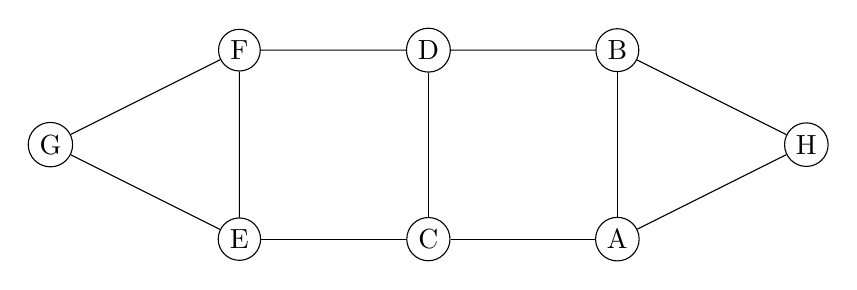
\begin{tikzpicture}[baseline=(current bounding box.center), scale=.8]
\tikzstyle{every node}=[circle, draw, fill=black!0,
                        inner sep=2pt, minimum width=10pt]
\path (0,0) node (A) {A} ;
\node (B)  at (-0,3) {B};
\node (C) at (-3,0) {C} ;
\node (E) at (-6,0) {E} ;
\node (F) at (-6,3)  {F} ;
\node (D) at (-3,3)  {D};
\node (G) at (-9, 1.5) {G};
\node (H) at (3,1.5) {H};
%\draw (D) edge[bend right=30] (F);
%\draw  (F) edge[bend right=30] (D);
%\draw (D)-- (E) --(C) --(A);
\foreach \i/\j in {A/B,B/D,A/C, C/D, C/E,E/F,A/H,B/H, D/F,G/F, G/E}{\draw (\i) -- (\j);}

\end{tikzpicture}

\bigskip

circuit: \hrulefill

\end{enumerate}
\end{document}

%-------------------------------------------------------------------------------------------------------------------------------------------------------------------------------------------------------------------

%%% Local Variables:
%%% mode: latex
%%% TeX-master: t
%%% End:
